\documentclass[]{beamer}

\usepackage{etoolbox}
\usepackage{xcolor}
\newtoggle{handout}
\togglefalse{handout}

\iftoggle{handout}{
	\usepackage{pgfpages}
	\pgfpagesuselayout{4 on 1}[border shrink=5mm]
}{}

\setbeamertemplate{footline}
{
	\hbox{\begin{beamercolorbox}[wd=1\paperwidth,ht=2.25ex,dp=1ex,right]{framenumber}%
			\usebeamerfont{framenumber}\insertframenumber{} / \inserttotalframenumber\hspace*{2ex}
	\end{beamercolorbox}}%
	\vskip0pt%
}

\definecolor{forest}{HTML}{154734}
\definecolor{miner}{HTML}{007A33}
\definecolor{lima}{HTML}{72BF44}
\definecolor{kiwi}{HTML}{BFD730}
\definecolor{mist}{HTML}{B1E4E3}

\setbeamertemplate{blocks}[rounded][shadow=true]
\setbeamertemplate{navigation symbols}{}
\setbeamercolor{frametitle}{fg=forest}
\setbeamercolor{structure}{fg=forest}
\setbeamercolor{block title}{bg=forest,fg=kiwi}
\setbeamercolor{block body}{bg=lima}

\usefonttheme{serif}


\usepackage{tikz}


\title{Bifurcation Analysis of a Discrete-Time Prey-Predator Model}
\author{by Pravaiz Naik, Zohreh Eskandari, Hossein Shahkari and Kolade Owolabi}
\institute{Presented by Jacob Hauck}
\date{}

\begin{document}
	\frame{\titlepage}
	
	\begin{frame}{Outline}
		\begin{itemize}
			\item Description and interpretation of a discrete-time predator-prey model
			\vfill
			\pause
			
			\item Determination of fixed points
			\vfill
			\pause
			
			\item Bifurcation analysis
			\begin{itemize}
				\item Period-doubling bifurcation
				\item Neimark-Sacker bifurcation
			\end{itemize}
			\vfill
			\pause
			
			\item Numerical investigations
			\begin{itemize}
				\item Bifurcation diagram of period-doubling bifurcation
				\item Phase portrait changes at Neimark-Sacker bifurcation
			\end{itemize}
		\end{itemize}
	\end{frame}
	
	\begin{frame}{Model Description}
		\begin{align*}
			x_p(n+1) &= x_p(n)\left[1 + r\left(1 - \frac{x_p(n)}{k}\right) - ay_p(n)\right] \\[0.3em]
			y_p(n+1) &= y_p(n)\left[1 - b + \frac{cx_p(n)}{y_p(n)}\right]
		\end{align*}
		\begin{itemize}
			\item $n \in \mathbb{Z}$: discrete time step
			\pause
			\item $x_p(n)$: number of prey; $y_p(n)$: number of predators
			\pause
			\item $r > 0$: intrinsic growth rate of prey
			\pause
			\item $k > 0$: carrying capacity of prey
			\pause
			\item $a > 0$: predation rate
			\pause
			\item $b > 0$: death rate of predators
			\pause
			\item $c > 0$: conversion rate (of prey into predators)
		\end{itemize}
	\end{frame}
	
	\begin{frame}{Fixed Points}
		$(0,0)$ is a fixed point (total extinction), and so is $(k,0)$ (predator extinction), but these are not the focus of the analysis.
		\vfill
		\pause
		
		Ecologically, an important fixed points occur when $x_p > 0$, and $y_p > 0$, when predator and prey are in equilibrium.
		\vfill
		\pause
		
		There is one such fixed point:
		\begin{equation*}
			\mathcal{P}_* = \left(\frac{rkb}{ack+br}, \frac{crk}{ack+br}\right).
		\end{equation*} 
	\end{frame}
	
	\begin{frame}{Period-doubling Bifurcations}
		On the time scale $\mathbb{Z}$, fixed points are also 1-periodic solutions. In general, if $x(n)$ is a solution of
		\begin{equation*}
			x(n+1) = f(x(n))
		\end{equation*}
		such that $x(n+p) = x(n)$, where $p$ is the smallest integer that makes this true, then $x_0 = x(0)$ is called a \textbf{periodic point of minimal period $p$}.
		\vfill
		\pause
		
		A \textbf{period-doubling bifurcation} occurs when the stability of a fixed point changes and a pair of periodic points of minimal period 2 emerge.
		\vfill
		\pause
		
		See Section 3.4 of \textit{Dynamics and Bifurcations}.
	\end{frame}
	
	\begin{frame}{Period-doubling Bifurcation in the Predator-Prey Model}
		\begin{block}{}
			Using the predation rate $a$ as a bifurcation parameter, there is a period-doubling bifurcation at the parameter value
			\begin{equation*}
				a_{\text{PD}} = -\frac{br(br-2b-2r+4)}{ck(br-2b+4)}.
			\end{equation*}
			Furthermore, the bifurcation is supercritical (subcritical) if $\widehat{\beta^{pp}_{\text{PD}}} > 0$ ($<0$), where
			\begin{equation*}
				\widehat{\beta^{pp}_{\text{PD}}} = \frac{16r(b-2)^3(r+2)}{(br-2b+4)^2k^2c^2(br-4)}.
			\end{equation*}
		\end{block}
		\vfill
		
		Recall: supercritical $\iff$ stable $\to$ unstable, subcritical $\iff$ unstable $\to$ stable.
	\end{frame}
	
	\begin{frame}{Period-Doubling Bifurcation -- Method}
		One-dimensional case (from \textit{Dynamics and Bifurcations}):
		
		\begin{block}{}
			Let $f \in C^3$ with
			\begin{equation*}
				f(0) = 0, \quad f'(0) = -1, \quad (f^2)'''(0) \ne 0.
			\end{equation*}
			If $F(\lambda, x)$ is a perturbation of $f$ such that
			\begin{equation*}
				F(0,x) = f(x), \quad F(\lambda,0)= 0, \quad \frac{\partial F}{\partial \lambda}(\lambda, 0) = -(1+\lambda),
			\end{equation*}
			then the discrete equation $x_{n+1} = F(\lambda, x_n)$ undergoes a period-doubling bifurcation at $\lambda = 0$.
		\end{block}
		\vfill
		
		Apply a similar result to higher-dimensional equations -- this involves Jacobian matrix and third-order partial derivatives.
	\end{frame}
	
	\begin{frame}{Period-Doubling Bifurcation Diagram}
		\begin{figure}
			\centering
			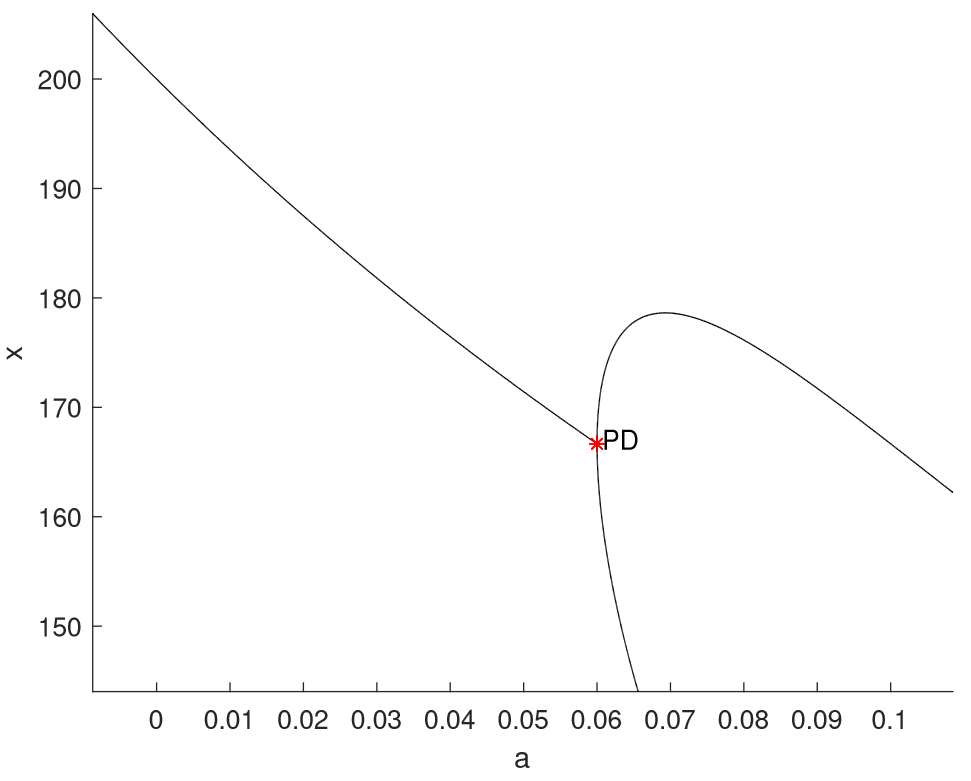
\includegraphics[width=.8\textwidth]{pd.png}
			
			A subcritical period-doubling bifurcation
		\end{figure}
	\end{frame}
	
	\begin{frame}{Neimark-Sacker Bifurcations}
		In a \textbf{Neimark-Sacker bifurcation} the fixed point changes stability type and a closed invariant curve containing the fixed point emerges with opposite stability.
		                                                                                      \vfill
		
		\begin{figure}
			\centering
			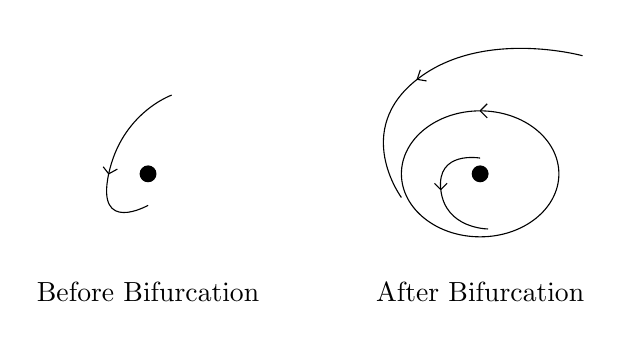
\begin{tikzpicture}
				\begin{scope}[xshift=-120]
				\draw[fill=black] (0,0) circle[radius=.1];
				\draw plot[smooth, tension=2] coordinates {(.3, 1) (-.5, 0) (0, -.4)};
				\draw (-.5,0) -- (-.57, .09);
				\draw (-.5,0) -- (-.39, .06);
				\node at (0,-1.5) {Before Bifurcation};
				\end{scope}
				
				\draw[fill=black] (0,0) circle[radius=.1];
				\draw (0,0) ellipse (1 and .8);
				\draw (0,.8) -- (.09, .89);
				\draw (0,.8) -- (.09, .71);
				\draw plot[smooth, tension=2] coordinates {(0,.2) (-.5, -.2) (.1, -.7)};
				\draw (-.5,-.2) -- (-.58, -.12);
				\draw (-.5,-.2) -- (-.42, -.12);
				\draw plot[smooth, tension=1.3] coordinates {(1.3, 1.5) (-.8,1.2) (-1, -.3)};
				\draw (-.8,1.2) -- (-.76,1.32);
				\draw (-.8,1.2) -- (-.68,1.18);
				\node at (0,-1.5) {After Bifurcation};
			\end{tikzpicture}
		\end{figure}
	\end{frame}
	
	\begin{frame}{Neimark-Sacker Bifurcation in the Predator-Prey Model}
		\begin{block}{}
			A Neimark-Sacker bifurcation occurs with respect to $a$ when
			\begin{equation*}
				a = a_{\text{NS}} = \frac{-r(br-b-r)}{ck(r-1)}.
			\end{equation*}
			The bifurcation is supercritical (subcritical) if $\widehat{\sigma^{pp}_{\text{NS}}} < 0$ ($>0$).
		\end{block}
		\vfill
		
		What is $\widehat{\sigma^{pp}_{\text{NS}}}$? This is a value that depends on the parameters and is related to the following result...
	\end{frame}
	
	\begin{frame}{Neimark-Sacker Bifurcation -- Method}
		From \textit{Elements of Applied Bifurcation Theory} by Y.A. Kuznetsov:
		\vfill
		\begin{block}{}
			In the two-dimensional discrete system $x_{n+1} = f(\lambda, x_n)$, let $\mu_{\pm}(\lambda) = r(\lambda)e^{\pm i\theta(\lambda)}$ be the eigenvalues of the Jacobian near $\lambda = 0$. If
			\begin{equation*}
				r(0) = 1, \quad r'(0) \ne 0, \quad e^{ik\theta(0)} \ne 1 \text{ for } k =1,2,3,4,
			\end{equation*}
			then the system undergoes a Neimark-Sacker bifurcation, which is supercritical (subcritical) if $\sigma = \Re\left(e^{-i\theta(0)}c_1(0)\right) < 0$ ($>0$).
		\end{block}
		\vfill
		
		Here, $c_1(0)$ is a complicated function of the first, second, and third derivatives of $f$ at $\lambda = 0$ and at the critical point.
	\end{frame}
	
	\begin{frame}{Phase Portraits Near the Neimark-Sacker Bifurcation}
		\begin{figure}
			\centering
			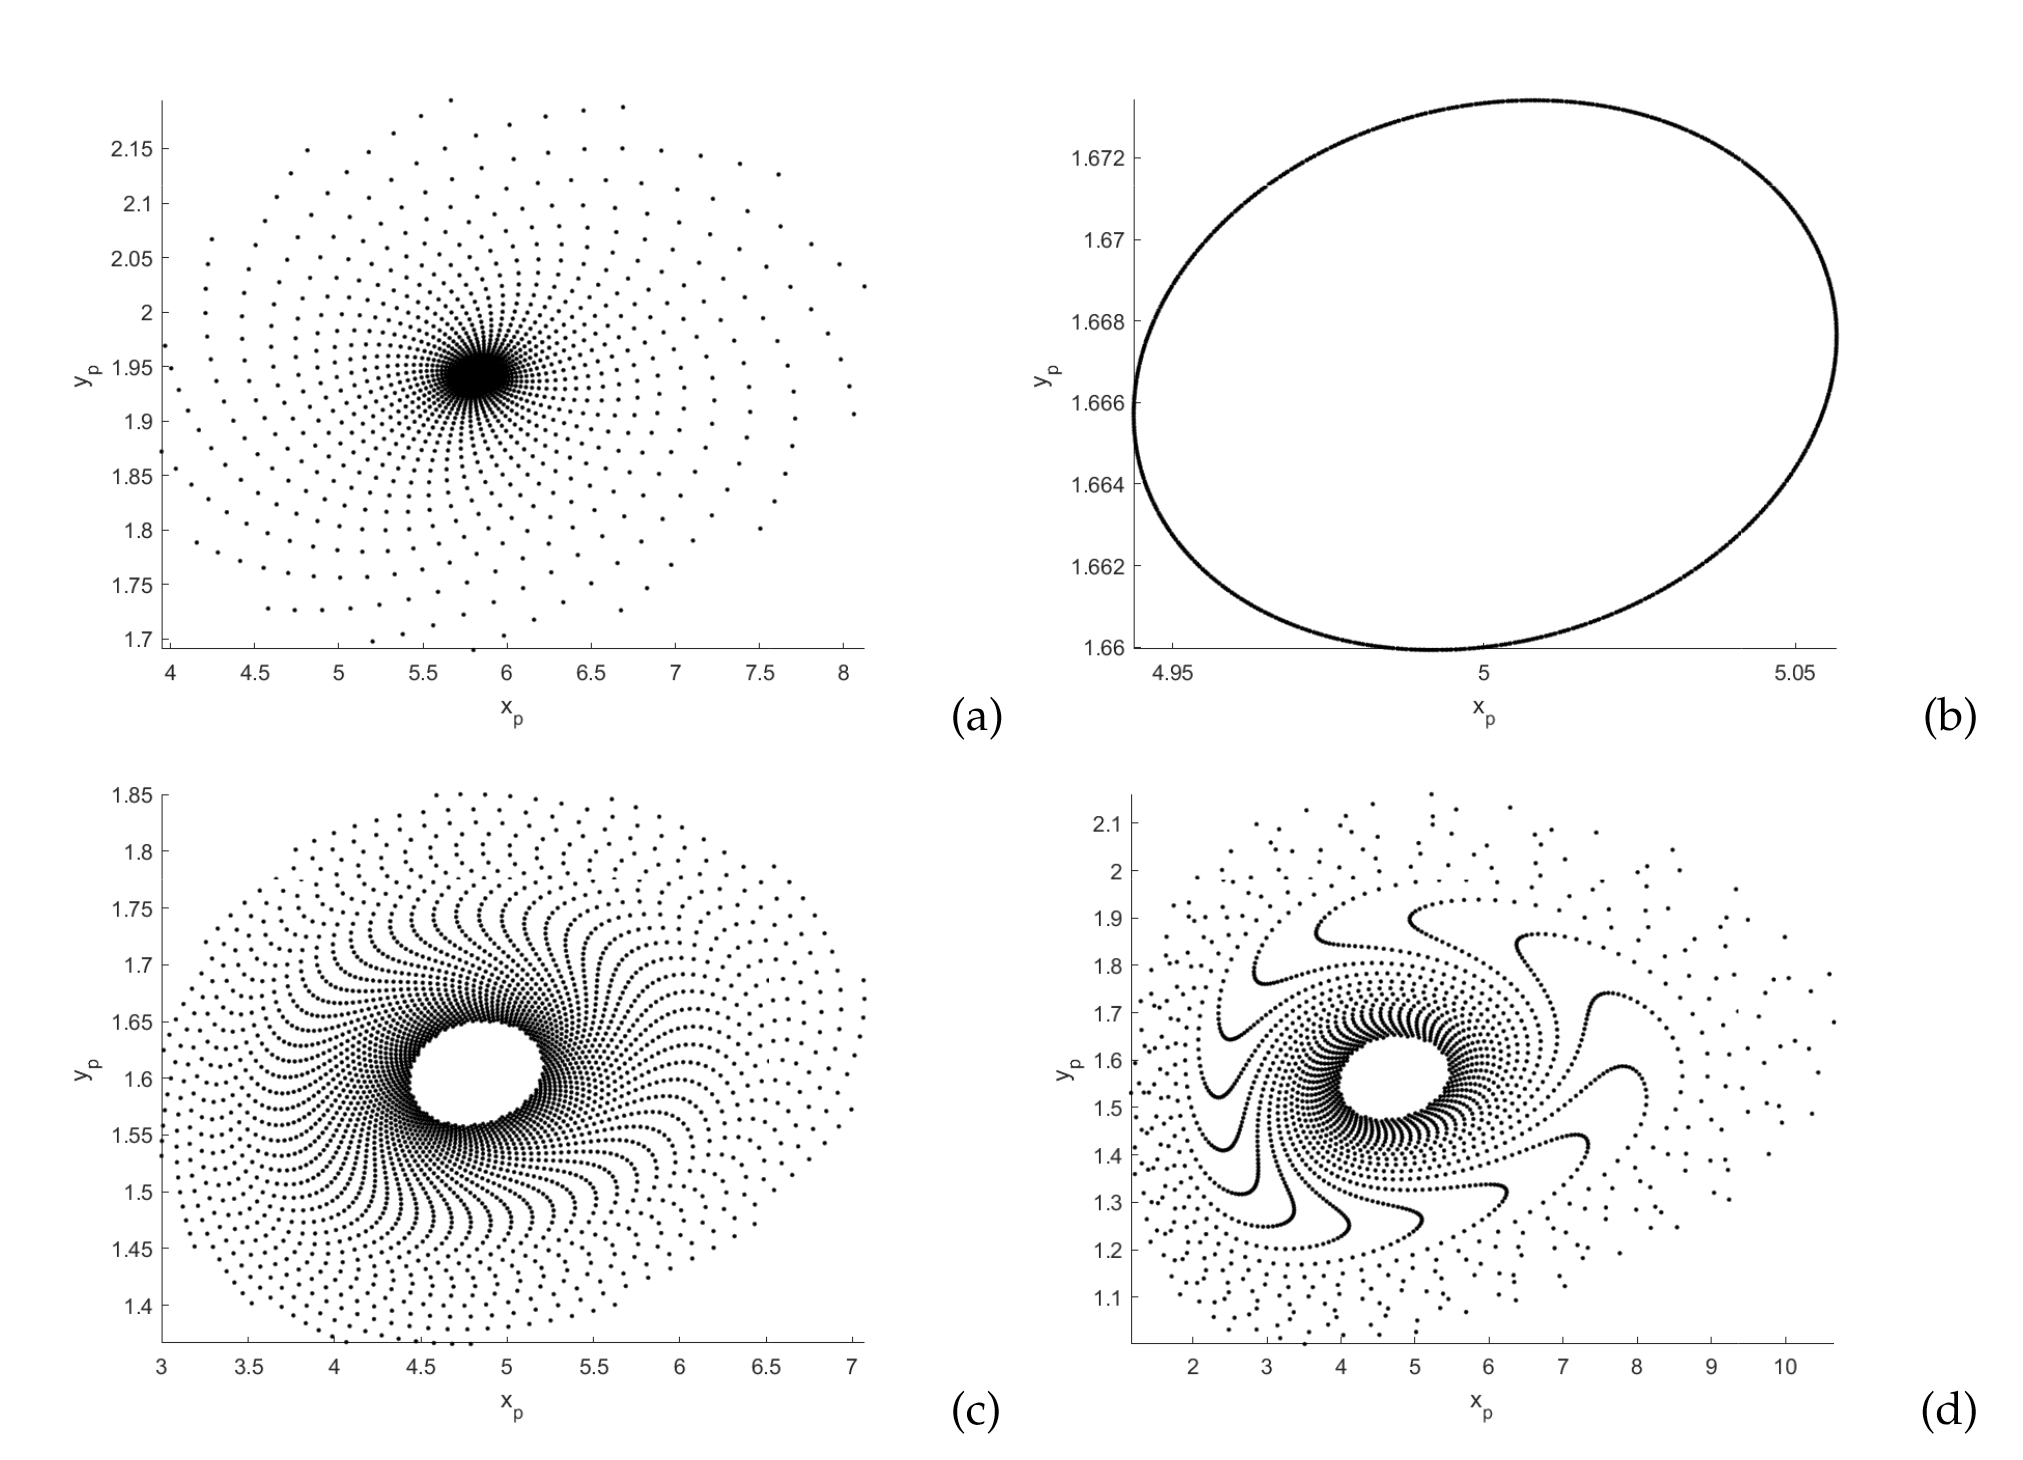
\includegraphics[width=\textwidth]{ns.png}
			
			(a) $a < a_{\text{NS}}$, (b) $a = a_{\text{NS}}$, (c) $a > a_{\text{NS}}$, (d) $a > a_{\text{NS}}$
		\end{figure}
	\end{frame}
	
	\iftoggle{handout}{}{
	\begin{frame}{}
		\centering
		Thank You!
	\end{frame}
	}
\end{document}